\documentclass[simple]{hfutexam}
\newcommand{\diff}{\,\mathrm{d}}
\usetikzlibrary{arrows.meta, overlay-beamer-styles}
\RequirePackage{extarrows}

\begin{document}
\BiaoTi{合肥工业大学期中试卷}
\XueNian{2021}{2022}
\XueQi{二}
\KeChengDaiMa{034Y01}
\KeChengMingCheng{数学(下)}
\XueFen{5}
\KeChengXingZhi{必修}
\KaoShiXingShi{闭卷}
\ZhuanYeBanJi{少数民族预科班}
\KaoShiRiQi{2022年5月13日8:00-10:00}
\MingTiJiaoShi{集体}
\maketitle

\begin{enumerate}
\item \textbf{(10分)} 求函数 $\displaystyle f(x)=\ln\frac1{\sqrt{x^2-1}}+\arctan\frac1x$ 的定义域.
\item \textbf{(5分)} 求函数 $\displaystyle y=\begin{cases}
1/x,&x<0,\\1,&x=0,\\1+e^{-x},&x>0\end{cases}$ 的反函数.
\item \textbf{(10分)} 求极限 $\displaystyle\lim_{x\to0^-}(1-x)^{1/x}$.
\item \textbf{(5分)} 求极限 $\displaystyle\lim_{x\to-2}\frac{x^2-4}{x^3+8}$.
\item \textbf{(5分)} 求极限 $\displaystyle\lim_{x\to0}\frac{\sin(e^{-x}-1)}{\arctan(1-\cos x)}$.
\item \textbf{(5分)} 求极限 $\displaystyle\lim_{x\to0}\frac{\sqrt{1+2x-x^2}-\sqrt{1-2x+x^2}}x$. 
\item \textbf{(5分)} 求极限 $\displaystyle\lim_{x\to\infty}\left(\cos\frac1x\right)^{\frac1{\ln(1+x^2)-2\ln x}}$.
\item \textbf{(5分)} 求极限 $\displaystyle\lim_{x\to\infty}\left(\frac\pi{e^x-1}-\arctan\frac x2\right)$. 
\item \textbf{(5分)} 求极限 $\displaystyle\lim_{n\to\infty}\left(\frac1{n^2+2}+\frac2{n^2+4}+\cdots+\frac n{n^2+2n}\right)$.
\item \textbf{(5分)} 设 $a_1=4,a_{n+1}=\sqrt{a_n+6}$, 证明 $\displaystyle\lim_{n\to\infty}a_n$ 存在并求之.
\item \textbf{(10分)} 证明 $e^x+x=4$ 在 $(0,+\infty)$ 内有零点.
\item \textbf{(5分)} 设函数 $f(x)$ 在 $[-1,1]$ 上连续, 且 $f(-1)\le1\le f(1)$. 证明存在 $\xi\in[-1,1]$, 使得 $f(\xi)=\xi^2$.
\item \textbf{(10分)} 求 $y=e^{x+1}\sin x-e^2\sin1$ 的导数.
\item \textbf{(5分)} 求 $y=\arctan e^x$ 的导数.
\item \textbf{(5分)} 求曲线 $y=\tan x$ 在点 $\left(-\dfrac\pi4,-1\right)$ 处的切线方程和法线方程.
\item \textbf{(5分)} 设
$\displaystyle f(x)=\begin{cases}\dfrac{e^{3x}-1}{\arctan x},&x<0,\\2x+a,&x\ge0\end{cases}$
在 $x=0$ 处连续, 求常数 $a$.
\end{enumerate}
\newpage

\BiaoTi{合肥工业大学试卷(A)}
\XueNian{2021}{2022}
\XueQi{二}
\KeChengDaiMa{034Y01}
\KeChengMingCheng{数学(下)}
\XueFen{5}
\KeChengXingZhi{必修}
\KaoShiXingShi{闭卷}
\ZhuanYeBanJi{少数民族预科班}
\KaoShiRiQi{2022年6月18日8:00-10:00}
\MingTiJiaoShi{集体}
\maketitle

\tigan{一、填空题(每题3分,共18分)}
\begin{enumerate}
\item 如果 $f(x)>0$ 且 $\displaystyle\lim_{x\to\infty}f(x)=0$, 则 $\displaystyle\lim_{x\to\infty}\bigl[1+f(x)\bigr]^{1/f(x)}=$\fillblank{}.
\item 设 $y=\sin(x^2+1)$, 则 $\diff y=$\fillblank{}.
\item 极限 $\displaystyle\lim_{n\to\infty}\left(\frac1{n^2-1}+\frac2{n^2-2}+\cdots+\frac n{n^2-n}\right)=$\fillblank{}.
\item 曲线 $y=2\ln(x+1)$ 在点 $(1,2\ln2)$ 处的切线方程为\fillblank{}.
\item 若 $e^{y-1}=1+xy$, 则 $\dfrac{\diff y}{\diff x}\bigg|_{x=0}=$\fillblank{}.
\item 如果函数 $f(x)$ 的定义域是 $(0,+\infty)$, 且 $x=0$ 是曲线 $y=f(x)$ 的垂直渐近线, 那么 $\displaystyle\lim_{x\to0^+}\frac1{f(x)}=$\fillblank{}.
\end{enumerate}

\tigan{二、选择题(每题3分,共18分)}
\begin{enumerate}
\item 当 $x\to+\infty$ 时, $\dfrac1x$ 和(~~~~)是等价无穷小.
\xx{$\sin\dfrac1x$}{$\sin x$}{$e^{-x}$}{$e^{1/x}$}
\item 若当 $x\to0$ 时, $\arctan(e^x-1)\cdot(\cos x-1)$ 和 $x^n$ 是同阶无穷小, 则 $n=$(~~~~).
\xx{$0$}{$1$}{$2$}{$3$}
\item 设 $f(x)=\arctan\dfrac1{x(x-1)^2}$, 则 $x=0$ 是 $f(x)$ 的(~~~~).
\xx{可去间断点}{跳跃间断点}{第二类间断点}{连续点}
\item
设 $f(x)$ 是定义在 $(-\infty,+\infty)$ 上的连续函数, 且 $f'(x)$ 的图像如下图所示, 则 $f(x)$ 有(~~~~).
\xx{一个极大值点,没有极小值点}{没有极大值点,一个极小值点}{一个极大值点和一个极小值点}{一个极大值点和两个极小值点}
\begin{center}
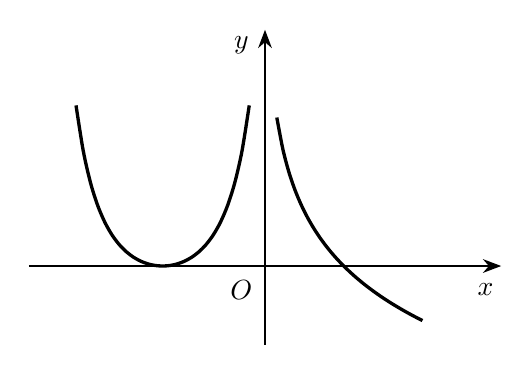
\begin{tikzpicture}
\draw[-Stealth,thick](-3,0)--(3,0);
\draw[-Stealth,thick](0,-1)--(0,3);
\draw[very thick,smooth,domain=-55:55] plot ({\x/50-1.3}, {tan(\x)*tan(\x)});
\draw[very thick,smooth,domain=0.15:2] plot ({\x}, {-ln(\x)});
\draw
	(-0.3,-0.3) node {$O$}
	(2.8,-0.3) node {$x$}
	(-0.3,2.8) node {$y$};
\end{tikzpicture}
\end{center}
\item 设 $f(x)$ 在点 $x=0$ 处可导, 且 $f(0)=0$, 则 $\displaystyle\lim_{x\to0}\frac{f(x^{2022})+x^{2021}f(x)}{x^{2022}}=$(~~~~).
\xx{$0$}{$f'(0)$}{$2f'(0)$}{$2022f'(0)$}
\item 如果点 $(x_0,y_0)$ 是曲线 $y=f(x)$ 的拐点, 则 $f''(x_0)=$(~~~~).
\xx{$0$}{$\infty$}{不存在}{$0$ 或不存在}
\end{enumerate}

\tigan{三、解答题(每题8分,共64分)}
\begin{enumerate}
\item 求极限 $\displaystyle\lim_{x\to-1}\frac{x^2-1}{x^2+3x+2}$.
\item 求极限 $\displaystyle\lim_{x\to0}\frac{e^x-1-x}{\arcsin x^2}$.
\item 设 $\begin{cases}x=t^2+t&\\y=t^3+t&\end{cases}$, 求 $\dfrac{\diff y}{\diff x}$ 和 $\dfrac{\diff^2 y}{\diff x^2}$.
\item 设 $f(x)=\begin{cases}x\arctan\dfrac1x,&x<0,\\x^2+ax+b,&x\ge0.\end{cases}$
求常数 $a,b$ 使得函数 $f(x)$ 在 $(-\infty,+\infty)$ 内可导, 并求出此时曲线 $y=f(x)$ 的渐近线.
\item	求函数 $f(x)=x^3-x^2-x$ 在区间 $[-2,2]$ 上的最大值和最小值.
\item 证明: 当 $-\dfrac\pi2<x_1<x_2<\dfrac\pi2$ 时, $\tan x_2-\tan x_1\ge x_2-x_1$.
\item 设函数 $f(x)$ 在 $(-\infty,+\infty)$ 内可导, 且 $f(1)=0$.
证明: 存在 $\xi\in(0,1)$ 使得 $\xi f'(\xi)+2022f(\xi)=0$.
\item 设函数 $f(x)=\ln x+\dfrac2{x^2}, x\in(0,+\infty)$. 求
\begin{enumerate}
\item[(1)] 函数 $f(x)$ 的增减区间及极值;
\item[(2)] 曲线 $y=f(x)$ 的凹凸区间及拐点.
\end{enumerate}
\end{enumerate}

\newpage
\BiaoTi{合肥工业大学试卷参考答案(A)}
\XueNian{2021}{2022}
\XueQi{二}
\KeChengDaiMa{034Y01}
\KeChengMingCheng{数学(下)}
\XueFen{5}
\KeChengXingZhi{必修}
\KaoShiXingShi{闭卷}
\ZhuanYeBanJi{少数民族预科班}
\KaoShiRiQi{2022年6月18日8:00-10:00}
\MingTiJiaoShi{集体}
\maketitle

\tigan{一、填空题(每小题3分,共18分)}

\textbf{请将你的答案对应填在横线上:}

\textbf{1.} \fillblank{$e$}, 
\textbf{2.} \fillblank{$2x\cos(x^2+1)\diff x$}, 
\textbf{3.} \fillblank{$1/2$}, \\
\textbf{4.} \fillblank{$y=x-1+2\ln 2$},
\textbf{5.} \fillblank{$1$},
\textbf{6.} \fillblank{$0$}.

\tigan{二、选择题(每小题3分,共18分)}

\textbf{请将你所选择的字母 A, B, C, D 之一对应填在下列表格里:}

\xuanzeti{\textbf{题号}}{\textbf{答案}}%
\xuanzeti{1}{A}%
\xuanzeti{2}{D}%
\xuanzeti{3}{B}%
\xuanzeti{4}{A}%
\xuanzeti{5}{C}%
\xuanzeti{6}{D}

\tigan{三、解答题(每小题8分,共64分)}

\textbf{1. (8分)【解】}
\vspace{-\baselineskip}

\begin{align*}
\lim_{x\to-1}\frac{x^2-1}{x^2+3x+2}&=\lim_{x\to-1}\frac{(x-1)(x+1)}{(x+2)(x+1)} \score3\\
&=\lim_{x\to-1}\frac{x-1}{x+2} \score3\\
&=\frac{-2}1=-2. \score2
\end{align*}

\textbf{2. (8分)【解】}
\vspace{-\baselineskip}

\begin{align*}
\lim_{x\to0}\frac{e^x-1-x}{\arcsin x^2}&=\lim_{x\to0}\frac{e^x-1-x}{x^2} \score3\\
&\xlongequal[]{\text{洛必达}}\lim_{x\to0}\frac{e^x-1}{2x} \score3\\
&=\lim_{x\to0}\frac{x}{2x}=\frac12. \score2
\end{align*}

\textbf{3. (8分)【解】}
\vspace{-\baselineskip}

\begin{align*}
\frac{\diff y}{\diff x}&=\frac{\diff y/\diff t}{\diff x/\diff t} \score2\\
&=\frac{3t^2+1}{2t+1}, \score2\\
\frac{\diff^2 y}{\diff x^2}&=\frac{\diff y'/\diff t}{\diff x/\diff t} \score2\\
&=\frac{6t(2t+1)-(3t^2+1)2}{(2t+1)^3}=\frac{6t^2+6t-2}{(2t+1)^3}. \score2
\end{align*}

\newpage
\textbf{4. (8分)【解】}

\indent 由于 $f(x)$ 在 $x=0$ 处连续, 因此
\begin{align*}
f(0)&=f(0^+) \score1\\
&=b=\lim_{x\to0^-}x\arctan\frac1x=0\times\left(-\frac\pi2\right)=0. \score1
\end{align*}

\indent 由于 $f(x)$ 在 $x=0$ 处可导, 因此
\begin{align*}
f'_-(0)&=f'_+(0), \score1\\
f'_-(0)&=\lim_{x\to0^-}\frac{x\arctan\frac1x}x=\lim_{x\to0^-}\arctan\frac1x=-\frac\pi2 \score1\\
f'_+(0)&=(2x+a)|_{x=0}=a, \score1
\end{align*}
因此 $a=-\dfrac\pi2$. \score1

\indent 由于
\begin{align*}
\lim_{x\to+\infty}\frac yx&=\lim_{x\to+\infty}\left(x-\frac\pi2\right)=+\infty, \score1\\
\lim_{x\to-\infty}\frac yx&=\lim_{x\to-\infty}\arctan\frac1x=0,\\
\lim_{x\to-\infty}y&=\lim_{x\to-\infty}x\arctan\frac1x=\lim_{t\to0^-}\frac{\arctan t}t=1,
\end{align*}
因此曲线 $y=f(x)$ 的渐近线只有 $y=1$. \score1

\textbf{5. (8分)【解】}

\indent 由
\[f'(x)=3x^2-2x-1=(3x+1)(x-1)=0 \score2\]
可得驻点 $x=-\dfrac13,1$. \score2

\indent 由于
\[f(-2)=-10,\quad f(2)=2,\quad f\left(-\frac13\right)=\frac5{27},\quad f(1)=-1, \score2\]
因此最大值为 $2$, 最小值为 $-10$. \score2

\textbf{6. (8分)【证明】}

\textbf{证法一}: 设 $f(x)=\tan x-x$, 则 \score2
\[f'(x)=\frac1{\cos^2x}-1=\tan^2x\ge0. \score2\]
因此 $f(x)$ 在 $\left(-\dfrac\pi2,\dfrac\pi2\right)$ 上单调递增, 从而 \score2
\[f(x_2)\ge f(x_1),\quad\tan x_2-\tan x_1\ge x_2-x_1. \score2\]

\newpage
\textbf{证法二}: 设 $f(x)=\tan x$, 则 $f(x)$ 在 $[x_1,x_2]$ 上连续, $(x_1,x_2)$ 内可导. \score2

\indent 由拉格朗日中值定理, 存在 $\xi\in(x_1,x_2)$ 使得
\[\frac{f(x_2)-f(x_1)}{x_2-x_1}=f'(\xi), \score2\]
即
\[\frac{\tan x_2-\tan x_1}{x_2-x_1}=\frac1{\cos^2\xi}\ge1. \score2\]
所以 $\tan x_2-\tan x_1\ge x_2-x_1$. \score2

\textbf{7. (8分)【证明】}

\indent 设 $F(x)=x^{2022}f(x)$, \score2\\
则 $F(x)$ 在 $[0,1]$ 上连续, $(0,1)$ 内可导, \score1\\
且 $F(0)=0,F(1)=f(1)=0$. \score1

\indent 由罗尔中值定理, 存在 $\xi\in(0,1)$ 使得 $F'(\xi)=0$. \score2\\
由于 $F'(x)=x^{2022}f'(x)+2022x^{2021}f(x)$ 且 $\xi\neq0$, \score1\\
所以 $\xi f'(\xi)+2022f(\xi)=1$. \score1


\textbf{8. (8分)【解】}

(1) 
\[f'(x)=\frac1x-\frac4{x^3}=\frac{x^2-4}{x^3}=\frac{(x+2)(x-2)}{x^3}. \score1\]
当 $0<x<2$ 时, $f'(x)<0$. 当 $x>2$ 时, $f'(x)>0$. \score1\\
因此 $(0,2]$ 是 $f(x)$ 的单减区间,\\
$[2,+\infty)$ 是 $f(x)$ 的单增区间. \Score{(1分, 写成开区间不扣分)}\\
所以 $f(x)$ 只有唯一的极小值 $f(2)=\ln2+\dfrac12$. \score1

(2) 
\[f''(x)=-\frac1{x^2}+\frac{12}{x^4}=-\frac{x^2-12}{x^4}=-\frac{(x-2\sqrt3)(x+2\sqrt3)}{x^4}. \score1\]
当 $0<x<2\sqrt3$ 时, $f''(x)>0$. 当 $x>2\sqrt3$ 时, $f''(x)<0$. \score1\\
因此 $(0,2\sqrt3]$ 是曲线 $y=f(x)$ 的凹区间,\\
$[2\sqrt3,+\infty)$ 是曲线 $y=f(x)$ 的凸区间,\Score{(1分, 写成开区间不扣分)}\\
拐点为 $\left(2\sqrt3,\ln(2\sqrt3)+\dfrac16\right)$. \score1

\end{document}




